{\bf Problem format was changed from original. Problem now have 15 seconds timelimit instead of unlimited interaction with environment and grader instead of library. }


The Black Box Game is played with a square-shaped black box lying flat on a table. Each of its four sides has $n$ holes (for a total of $4\cdot n$ holes) into which a ball can be thrown. A thrown ball will eventually exit from one of the $4\cdot n$ holes, potentially the same hole into which it was thrown. 

The black box's internals can be envisioned as an $n \times n$ grid. The 
holes in the sides are the starts and ends of rows and columns.  Each of the box's squares is either empty or occupied by a deflector. A deflector is a piece of hardware that changes the direction of the ball by 90 degrees. Consider this example of a $5 \times 5$ box. 

\begin{center}
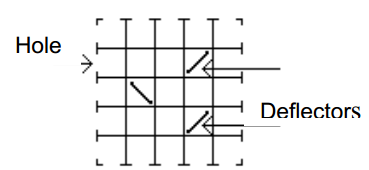
\includegraphics[bb=0 0 275 110]{blackbox1.png}
\end{center}

A ball thrown into the box follows a straight line until it either hits a deflector or exits the box. When a ball hits a deflector, the ball changes direction and the deflector toggles its position (by ``toggle'' we mean rotate 90 degrees). The examples below show the action of a deflector. 

\begin{center}
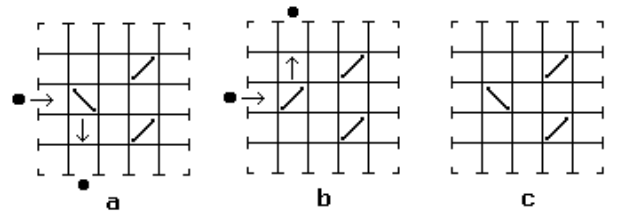
\includegraphics[bb=0 0 600 150]{blackbox2.png}
\end{center}

\begin{enumerate}
\item A ball is thrown through a hole; it hits a deflector and changes direction. 
\item After the first ball was thrown, the deflector has toggled its position. A new ball is thrown into the same hole, hits the deflector and is deflected in a direction opposite to that of the first ball. 
\item  The deflector toggles every time it is hit.
\end{enumerate}

Whenever a deflector is hit, it makes a beep. The number of times the ball was deflected can be deduced by counting the beeps. It can be proved that the ball always exits the box. The box has a button that resets it to its original state and another button that toggles all of its deflectors. 

You will be provided with an interface to black box via grader. You must determine the internals of the box as best as possible . 


$1 \le n \le 30$